% Options for packages loaded elsewhere
\PassOptionsToPackage{unicode}{hyperref}
\PassOptionsToPackage{hyphens}{url}
%
\documentclass[
  11pt]{report}
\usepackage{amsmath,amssymb}
\usepackage{lmodern}
\usepackage{iftex}
\ifPDFTeX
  \usepackage[T1]{fontenc}
  \usepackage[utf8]{inputenc}
  \usepackage{textcomp} % provide euro and other symbols
\else % if luatex or xetex
  \usepackage{unicode-math}
  \defaultfontfeatures{Scale=MatchLowercase}
  \defaultfontfeatures[\rmfamily]{Ligatures=TeX,Scale=1}
\fi
% Use upquote if available, for straight quotes in verbatim environments
\IfFileExists{upquote.sty}{\usepackage{upquote}}{}
\IfFileExists{microtype.sty}{% use microtype if available
  \usepackage[]{microtype}
  \UseMicrotypeSet[protrusion]{basicmath} % disable protrusion for tt fonts
}{}
\makeatletter
\@ifundefined{KOMAClassName}{% if non-KOMA class
  \IfFileExists{parskip.sty}{%
    \usepackage{parskip}
  }{% else
    \setlength{\parindent}{0pt}
    \setlength{\parskip}{6pt plus 2pt minus 1pt}}
}{% if KOMA class
  \KOMAoptions{parskip=half}}
\makeatother
\usepackage{xcolor}
\IfFileExists{xurl.sty}{\usepackage{xurl}}{} % add URL line breaks if available
\IfFileExists{bookmark.sty}{\usepackage{bookmark}}{\usepackage{hyperref}}
\hypersetup{
  pdftitle={Introduction to Stochastic Processes With R, by Robert P. Dobrow},
  pdfauthor={Fernando Náufel},
  pdflang={en},
  hidelinks,
  pdfcreator={LaTeX via pandoc}}
\urlstyle{same} % disable monospaced font for URLs
\usepackage[margin=1in]{geometry}
\usepackage{color}
\usepackage{fancyvrb}
\newcommand{\VerbBar}{|}
\newcommand{\VERB}{\Verb[commandchars=\\\{\}]}
\DefineVerbatimEnvironment{Highlighting}{Verbatim}{commandchars=\\\{\}}
% Add ',fontsize=\small' for more characters per line
\usepackage{framed}
\definecolor{shadecolor}{RGB}{248,248,248}
\newenvironment{Shaded}{\begin{snugshade}}{\end{snugshade}}
\newcommand{\AlertTok}[1]{\textcolor[rgb]{0.94,0.16,0.16}{#1}}
\newcommand{\AnnotationTok}[1]{\textcolor[rgb]{0.56,0.35,0.01}{\textbf{\textit{#1}}}}
\newcommand{\AttributeTok}[1]{\textcolor[rgb]{0.77,0.63,0.00}{#1}}
\newcommand{\BaseNTok}[1]{\textcolor[rgb]{0.00,0.00,0.81}{#1}}
\newcommand{\BuiltInTok}[1]{#1}
\newcommand{\CharTok}[1]{\textcolor[rgb]{0.31,0.60,0.02}{#1}}
\newcommand{\CommentTok}[1]{\textcolor[rgb]{0.56,0.35,0.01}{\textit{#1}}}
\newcommand{\CommentVarTok}[1]{\textcolor[rgb]{0.56,0.35,0.01}{\textbf{\textit{#1}}}}
\newcommand{\ConstantTok}[1]{\textcolor[rgb]{0.00,0.00,0.00}{#1}}
\newcommand{\ControlFlowTok}[1]{\textcolor[rgb]{0.13,0.29,0.53}{\textbf{#1}}}
\newcommand{\DataTypeTok}[1]{\textcolor[rgb]{0.13,0.29,0.53}{#1}}
\newcommand{\DecValTok}[1]{\textcolor[rgb]{0.00,0.00,0.81}{#1}}
\newcommand{\DocumentationTok}[1]{\textcolor[rgb]{0.56,0.35,0.01}{\textbf{\textit{#1}}}}
\newcommand{\ErrorTok}[1]{\textcolor[rgb]{0.64,0.00,0.00}{\textbf{#1}}}
\newcommand{\ExtensionTok}[1]{#1}
\newcommand{\FloatTok}[1]{\textcolor[rgb]{0.00,0.00,0.81}{#1}}
\newcommand{\FunctionTok}[1]{\textcolor[rgb]{0.00,0.00,0.00}{#1}}
\newcommand{\ImportTok}[1]{#1}
\newcommand{\InformationTok}[1]{\textcolor[rgb]{0.56,0.35,0.01}{\textbf{\textit{#1}}}}
\newcommand{\KeywordTok}[1]{\textcolor[rgb]{0.13,0.29,0.53}{\textbf{#1}}}
\newcommand{\NormalTok}[1]{#1}
\newcommand{\OperatorTok}[1]{\textcolor[rgb]{0.81,0.36,0.00}{\textbf{#1}}}
\newcommand{\OtherTok}[1]{\textcolor[rgb]{0.56,0.35,0.01}{#1}}
\newcommand{\PreprocessorTok}[1]{\textcolor[rgb]{0.56,0.35,0.01}{\textit{#1}}}
\newcommand{\RegionMarkerTok}[1]{#1}
\newcommand{\SpecialCharTok}[1]{\textcolor[rgb]{0.00,0.00,0.00}{#1}}
\newcommand{\SpecialStringTok}[1]{\textcolor[rgb]{0.31,0.60,0.02}{#1}}
\newcommand{\StringTok}[1]{\textcolor[rgb]{0.31,0.60,0.02}{#1}}
\newcommand{\VariableTok}[1]{\textcolor[rgb]{0.00,0.00,0.00}{#1}}
\newcommand{\VerbatimStringTok}[1]{\textcolor[rgb]{0.31,0.60,0.02}{#1}}
\newcommand{\WarningTok}[1]{\textcolor[rgb]{0.56,0.35,0.01}{\textbf{\textit{#1}}}}
\usepackage{longtable,booktabs,array}
\usepackage{calc} % for calculating minipage widths
% Correct order of tables after \paragraph or \subparagraph
\usepackage{etoolbox}
\makeatletter
\patchcmd\longtable{\par}{\if@noskipsec\mbox{}\fi\par}{}{}
\makeatother
% Allow footnotes in longtable head/foot
\IfFileExists{footnotehyper.sty}{\usepackage{footnotehyper}}{\usepackage{footnote}}
\makesavenoteenv{longtable}
\setlength{\emergencystretch}{3em} % prevent overfull lines
\providecommand{\tightlist}{%
  \setlength{\itemsep}{0pt}\setlength{\parskip}{0pt}}
\setcounter{secnumdepth}{5}
\newlength{\cslhangindent}
\setlength{\cslhangindent}{1.5em}
\newlength{\csllabelwidth}
\setlength{\csllabelwidth}{3em}
\newlength{\cslentryspacingunit} % times entry-spacing
\setlength{\cslentryspacingunit}{\parskip}
\newenvironment{CSLReferences}[2] % #1 hanging-ident, #2 entry spacing
 {% don't indent paragraphs
  \setlength{\parindent}{0pt}
  % turn on hanging indent if param 1 is 1
  \ifodd #1
  \let\oldpar\par
  \def\par{\hangindent=\cslhangindent\oldpar}
  \fi
  % set entry spacing
  \setlength{\parskip}{#2\cslentryspacingunit}
 }%
 {}
\usepackage{calc}
\newcommand{\CSLBlock}[1]{#1\hfill\break}
\newcommand{\CSLLeftMargin}[1]{\parbox[t]{\csllabelwidth}{#1}}
\newcommand{\CSLRightInline}[1]{\parbox[t]{\linewidth - \csllabelwidth}{#1}\break}
\newcommand{\CSLIndent}[1]{\hspace{\cslhangindent}#1}
\ifLuaTeX
\usepackage[bidi=basic]{babel}
\else
\usepackage[bidi=default]{babel}
\fi
\babelprovide[main,import]{english}
% get rid of language-specific shorthands (see #6817):
\let\LanguageShortHands\languageshorthands
\def\languageshorthands#1{}

% A command to save the path to the resources of bd.format (fnaufel)
\newcommand{\dir}{/ssd/R/x86_64-pc-linux-gnu-library/4.1/fnaufelRmd/rmarkdown/resources}



\hypersetup{
  colorlinks,
  breaklinks,
  linkcolor=magenta,
  urlcolor=blue
}

% Lexend font
\usepackage{lexend}


% Para bibliografia em português
\usepackage{babelbib}

% Para títulos de capítulos e seções:
\usepackage[nobottomtitles*]{titlesec}

%%%%%%%%%%%%%%%
%
% Titulos de capítulos e seções

\titleformat{\chapter}[display]%
{\bfseries\Large}%
{\filleft\MakeUppercase{\chaptertitlename} \Huge\thechapter}%
{4ex}%
{\titlerule%
  \vspace{2ex}%
  \filright}%
[\vspace{2ex}%
\titlerule%
\vspace{10ex}]

\titleformat{\section}[block]%
{\bfseries\Large}%
{\thesection}{.5em}{\titlerule\\[.8ex]\bfseries}

\titleformat{\subsection}[block]%
{\bfseries}%
{\thesubsection}{.5em}{\titlerule\\[.8ex]\bfseries}%
[\vspace{1ex}]

\titleformat{\subsubsection}[block]%
{\itshape}%
{\thesubsubsection}{.5em}{\titlerule\\[.8ex]\itshape}%
[\vspace{1ex}]

\titleformat{\paragraph}[block]%
{\itshape}%
{\theparagraph}{.5em}{\\[.8ex]\itshape}%
[\vspace{1ex}]


%%%%%%%%%%%%%%%
%
% Caixas

\usepackage{tcolorbox}
\tcbuselibrary{breakable}
\tcbuselibrary{skins}

\tcbset{
  enhanced,
  rounded corners,
  boxrule=0.3mm,
  colback=black!.5!white,
  parbox=false,
  /tcb/breakable=true
}

\newtcolorbox{rmdbox}{
  colframe=black!40!white,
}


\newtcolorbox{mycaution}{
  colframe=red!75!black,
  sidebyside,
  lower separated=false,
  lefthand width=1cm,
  sidebyside gap=4mm
}

\newenvironment{rmdcaution}
{
  \begin{mycaution}
    
\includegraphics[width=.8cm]{\dir/images/caution.png}
    \tcblower
  }
  {
  \end{mycaution}
}

\newtcolorbox{myimportant}{
  colframe=green!75!black,
  sidebyside,
  lower separated=false,
  lefthand width=1cm,
  sidebyside gap=4mm
}

\newenvironment{rmdimportant}
{
  \begin{myimportant}
    
\includegraphics[width=.8cm]{\dir/images/important.png}
    \tcblower
  }
  {
  \end{myimportant}
}

\newtcolorbox{mywarning}{
  colframe=yellow!80!black,
  sidebyside,
  lower separated=false,
  lefthand width=1cm,
  sidebyside gap=4mm
}

\newenvironment{rmdwarning}
{
  \begin{mywarning}
    
\includegraphics[width=.8cm]{\dir/images/warning.png}
    \tcblower
  }
  {
  \end{mywarning}
}

\newtcolorbox{mynote}{
  colframe=yellow!70!black,
  sidebyside,
  lower separated=false,
  lefthand width=1cm,
  sidebyside gap=4mm
}

\newenvironment{rmdnote}
{
  \begin{mynote}
    
\includegraphics[width=.8cm]{\dir/images/note.png}
    \tcblower
  }
  {
  \end{mynote}
}

\newtcolorbox{mytip}{
  colframe=blue!50!white,
  sidebyside,
  lower separated=false,
  lefthand width=1cm,
  sidebyside gap=4mm
}

\newenvironment{rmdtip}
{
  \begin{mytip}
    
\includegraphics[width=.8cm]{\dir/images/tip.png}
    \tcblower
  }
  {
  \end{mytip}
}

% For highlighting using \hl{}
\usepackage{soul}


\makeatletter
\@ifundefined{Shaded}{}{
  % Code chunks and output
  \usepackage[framemethod=pgf]{mdframed}
  \renewenvironment{Shaded}{
    \begin{mdframed}[%
      roundcorner=2pt,%
      innerleftmargin=5pt,%
      innerrightmargin=5pt,%
      topline=true,%
      leftline=true,%
      rightline=true,%
      bottomline=true,%
      linewidth=0.5pt,%
      linecolor=black!20,%
      backgroundcolor=black!2,%
      skipabove=2ex,%
      skipbelow=2.5ex%
    ]%
  }
  {
    \end{mdframed}
  }
}
\makeatother

% Use tt in tables
\usepackage{longtable}
\let\oldlongtable\longtable
\let\endoldlongtable\endlongtable
\renewenvironment{longtable}{\tt\oldlongtable}{\endoldlongtable}


% End of preamble for bookdowntemplate01

%%%%%%%%%%%%%%%%%%%%%%%%%%%%%%%%%%%%%%%%%%%%%%%%%%%%%%

\usepackage{booktabs}
\usepackage{longtable}
\usepackage{array}
\usepackage{multirow}
\usepackage{wrapfig}
\usepackage{float}
\usepackage{colortbl}
\usepackage{pdflscape}
\usepackage{tabu}
\usepackage{threeparttable}
\usepackage{threeparttablex}
\usepackage[normalem]{ulem}
\usepackage{makecell}
\usepackage{xcolor}
\ifLuaTeX
  \usepackage{selnolig}  % disable illegal ligatures
\fi

\title{Introduction to Stochastic Processes With R, by Robert P. Dobrow}
\author{Fernando Náufel}
\date{21/04/2022}

\begin{document}
\maketitle

{
\setcounter{tocdepth}{1}
\tableofcontents
}
\hypertarget{presentation}{%
\chapter*{Presentation}\label{presentation}}
\addcontentsline{toc}{chapter}{Presentation}

Notes about (\protect\hyperlink{ref-RobertP.Dobrow1345}{Dobrow 2016}).

\hypertarget{introduction-and-review}{%
\chapter{Introduction and review}\label{introduction-and-review}}

\hypertarget{deterministic-and-stochastic-models}{%
\section{Deterministic and Stochastic Models}\label{deterministic-and-stochastic-models}}

\hypertarget{example-1.2-sir-model}{%
\subsection*{Example 1.2 (SIR model)}\label{example-1.2-sir-model}}
\addcontentsline{toc}{subsection}{Example 1.2 (SIR model)}

\begin{rmdbox}

\begin{itemize}
\item
  $S_t = {}$ number of {\hl{susceptible}} people at time $t$.
\item
  $I_t = {}$ number of {\hl{newly infected}} people at time $t$.
\item
  $R_t = {}$ number of {\hl{recovered}} people at time $t$.
\item
  $z = {}$ probability that a {\hl{susceptible}} individual {\hl{becomes infected}} once in contact with an infected person.
\item
  Assume every susceptible person comes in contact with every infected person.
\end{itemize}

\end{rmdbox}

\begin{itemize}
\item
  Probability $p$ that a susceptible individual becomes infected at a point in time:

  \[
  p_t = 1 - (1 - z)^{I_{t-1}}
  \]

  \begin{rmdwarning}
  The book has the exponent as $I_{t}$, but the correct exponent is $I_{t - 1}$.

  In this discrete time model, we compute the number of newly infected people as a function of the number of people infected at the previous time step.

  \end{rmdwarning}
\item
  This is because $(1 - z)^{I_{t - 1}}$ is the probability that the person has contact with all $I_{t-1}$ infected people and {\hl{does not become infected}}.
\item
  The number of newly infected people $I_{t}$ follows a binomial distribution with $n = S_{t-1}$ and probability of success $p_t$:

  \[
  I_{t} \sim \text{Bin}(S_{t-1}, p_t)
  \]

  so the PMF is

  \[
  P(I_{t} = k) = \binom{S_{t-1}}{k} \; p_t^k \; (1 - p_t)^{S_{t-1} - k}
  \]
\item
  Then the number of susceptible people at time $t$ is

  \[
  S_{t} = S_{t-1} - I_{t}
  \]
\item
  This simplified example does not take into account the transition from infected to recovered.
\item
  $I_t$ is the number of \emph{newly} infected people at time $t$.
\item
  In the computation, only newly infected people are contagious. It's as if people remain infected and contagious for one time step only.
\end{itemize}

\hypertarget{simulations}{%
\subsubsection*{Simulations}\label{simulations}}
\addcontentsline{toc}{subsubsection}{Simulations}

\begin{center}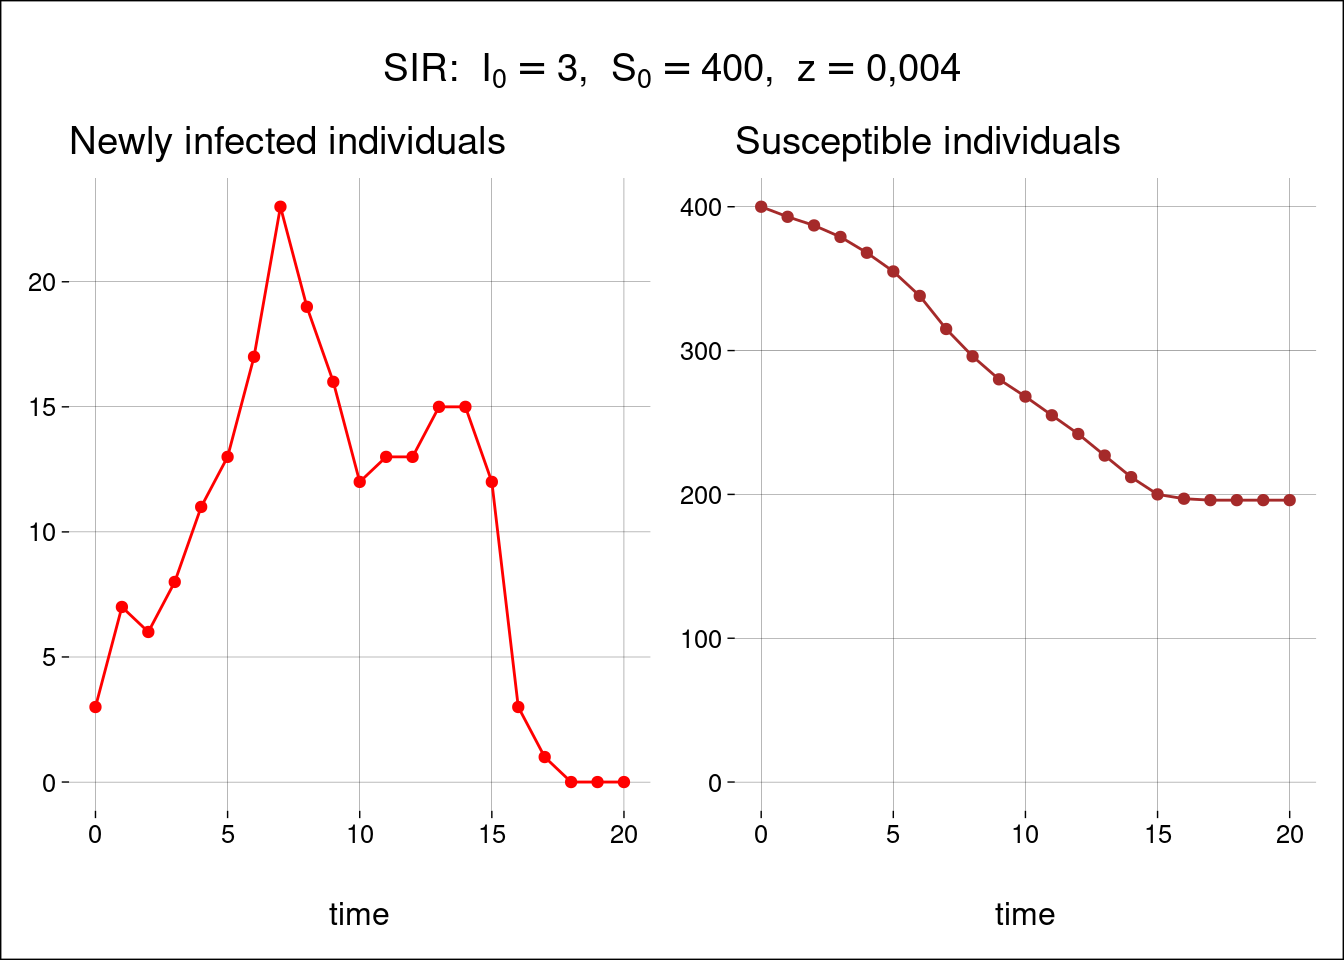
\includegraphics[width=1\linewidth]{_main_files/figure-latex/unnamed-chunk-4-1} \end{center}

\begin{center}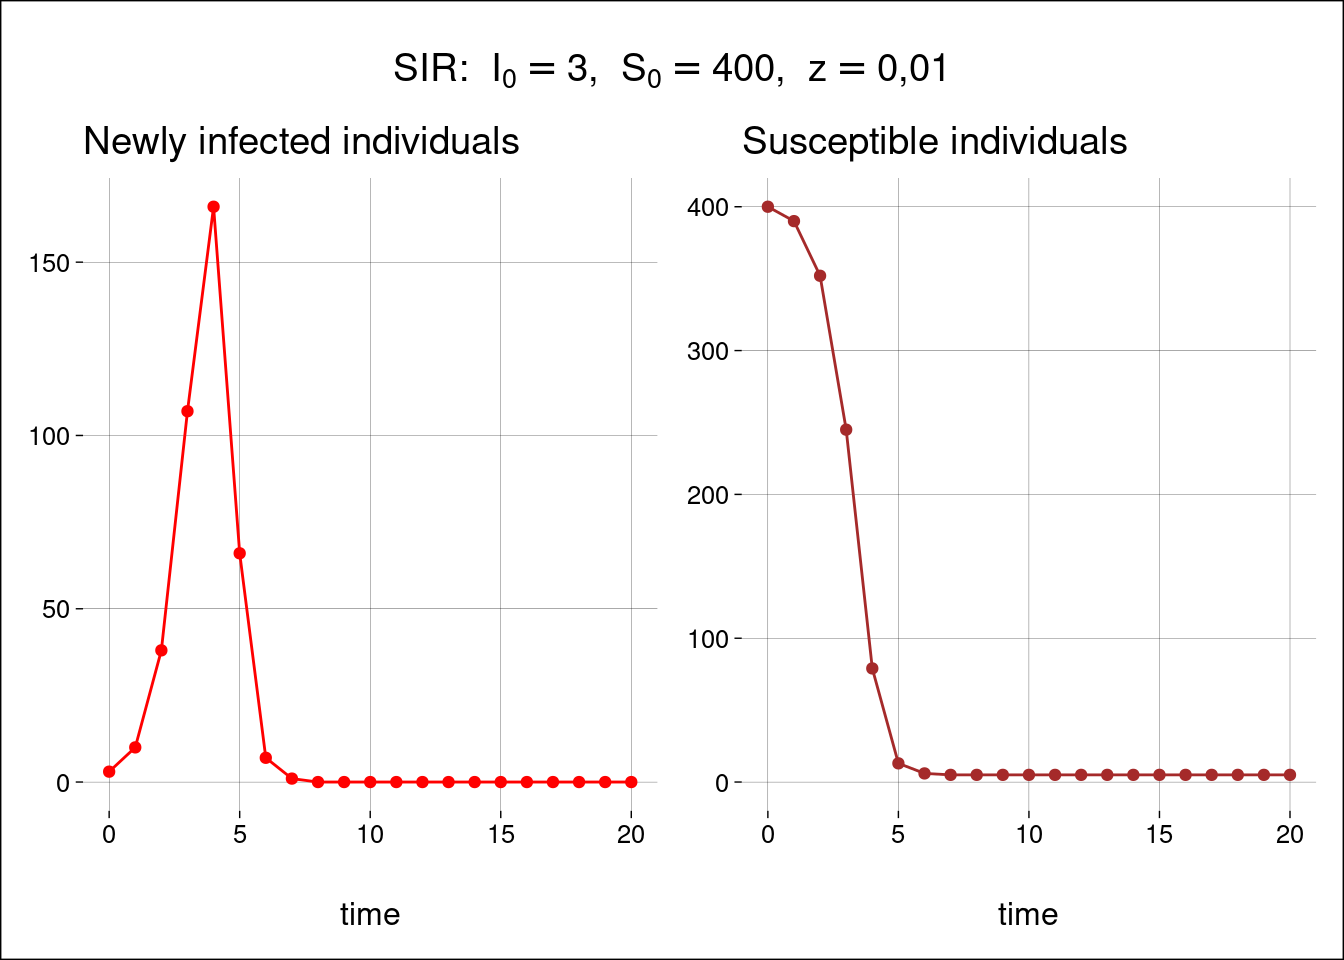
\includegraphics[width=1\linewidth]{_main_files/figure-latex/unnamed-chunk-5-1} \end{center}

\begin{center}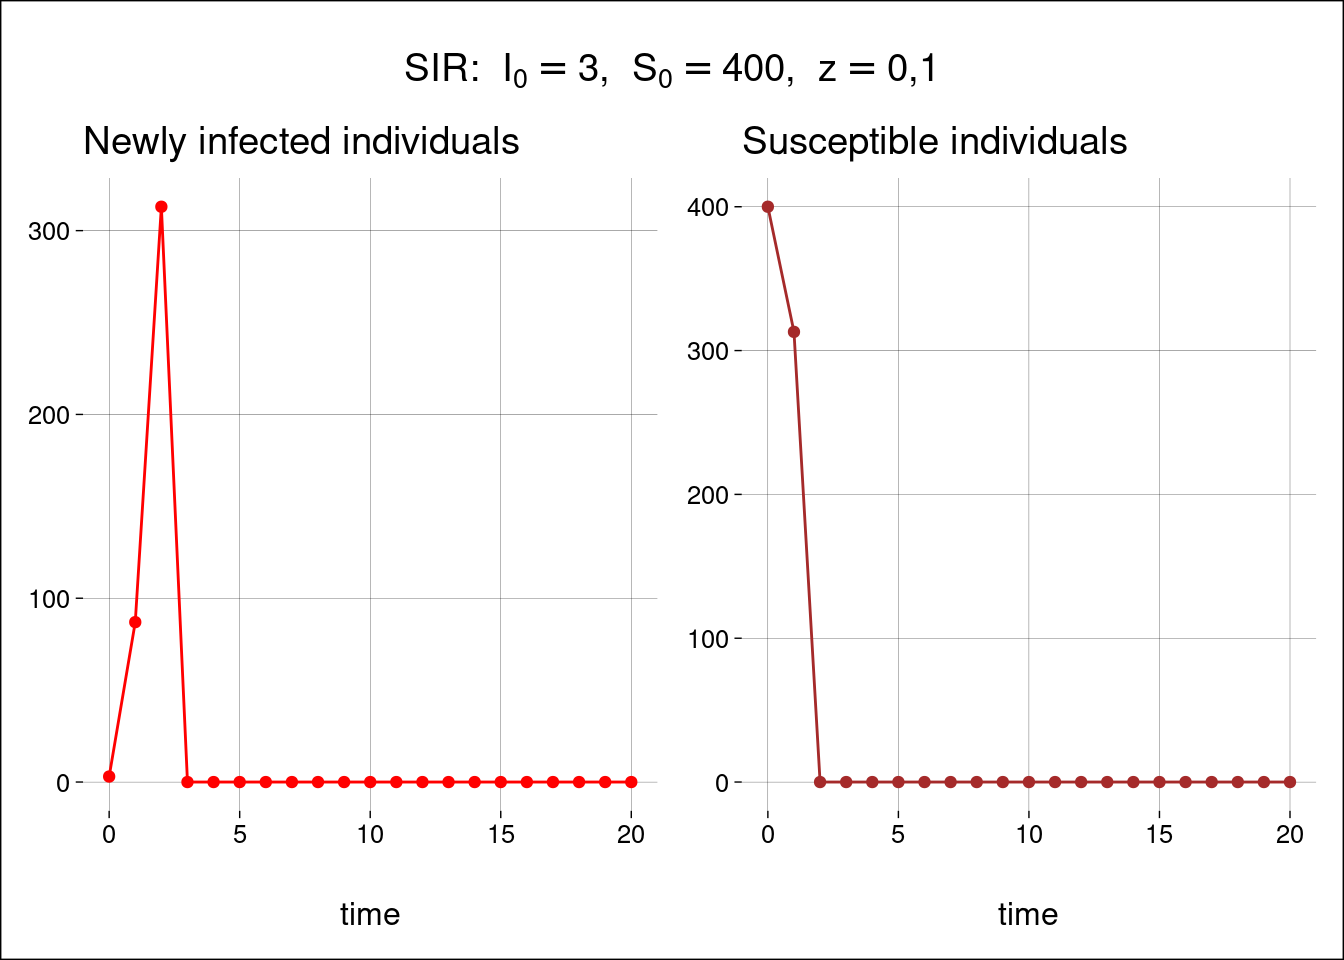
\includegraphics[width=1\linewidth]{_main_files/figure-latex/unnamed-chunk-6-1} \end{center}

\begin{center}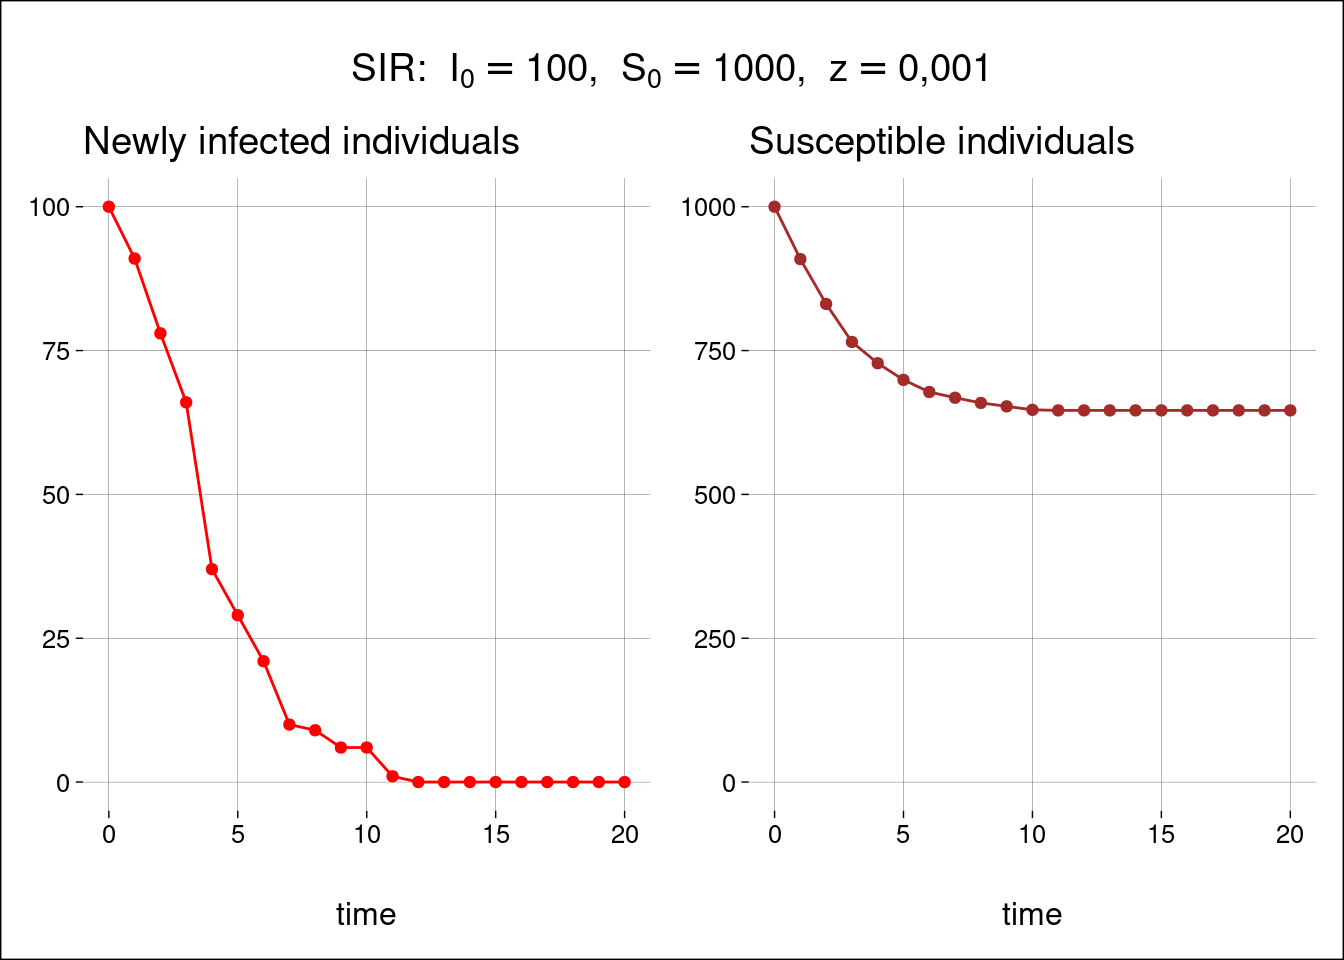
\includegraphics[width=1\linewidth]{_main_files/figure-latex/unnamed-chunk-7-1} \end{center}

\hypertarget{what-is-a-stochastic-process}{%
\section{What is a stochastic process?}\label{what-is-a-stochastic-process}}

\hypertarget{example-1.6-random-walk-and-gamblers-ruin}{%
\subsection*{Example 1.6 (Random walk and gambler's ruin)}\label{example-1.6-random-walk-and-gamblers-ruin}}
\addcontentsline{toc}{subsection}{Example 1.6 (Random walk and gambler's ruin)}

\ldots{}

\hypertarget{prob-review}{%
\chapter*{Appendix B: Probability review}\label{prob-review}}
\addcontentsline{toc}{chapter}{Appendix B: Probability review}

\hypertarget{b.4-common-probability-distributions}{%
\section*{B.4 Common probability distributions}\label{b.4-common-probability-distributions}}
\addcontentsline{toc}{section}{B.4 Common probability distributions}

\hypertarget{bivariate-normal}{%
\subsection*{Bivariate normal}\label{bivariate-normal}}
\addcontentsline{toc}{subsection}{Bivariate normal}

\begin{itemize}
\item
  The bivariate normal is defined here through its PDF --- which is {\hl{not}} given in its general form, but only in the case where $X \sim \mathcal N(0, 1)$ and $Y \sim \mathcal N(0, 1)$:

  \[
  f(x, y) = \frac{1}{2\pi\tau} \cdot 
  \exp\left(
    -\frac{1}{2\tau^2} \cdot (x^2 - 2\rho xy + y^2)
  \right)
  \]

  with $\tau = \sqrt{1 - \rho^2}$, where $\rho$ is the {\hl{correlation}} between $X$ and $Y$.
\item
  If the marginal distributions of $X$ and $Y$ are given, $\rho$ is still free to vary in $[-1, 1]$.
\item
  So, there are {\hl{five parameters}}: $\mu_X$, $\sigma_X$, $\mu_Y$, $\sigma_Y$, and $\rho$.
\item
  This figure from (\protect\hyperlink{ref-JosephK.Blitzstein989}{Blitzstein and Hwang 2019}) shows two bivariate normals with the same marginal distributions (the standard univariate normal) but different correlations $\rho$:

\begin{Shaded}
\begin{Highlighting}[]
\NormalTok{knitr}\SpecialCharTok{::}\FunctionTok{include\_graphics}\NormalTok{(}\StringTok{\textquotesingle{}images/bvn.jpg\textquotesingle{}}\NormalTok{)}
\end{Highlighting}
\end{Shaded}

  \begin{center}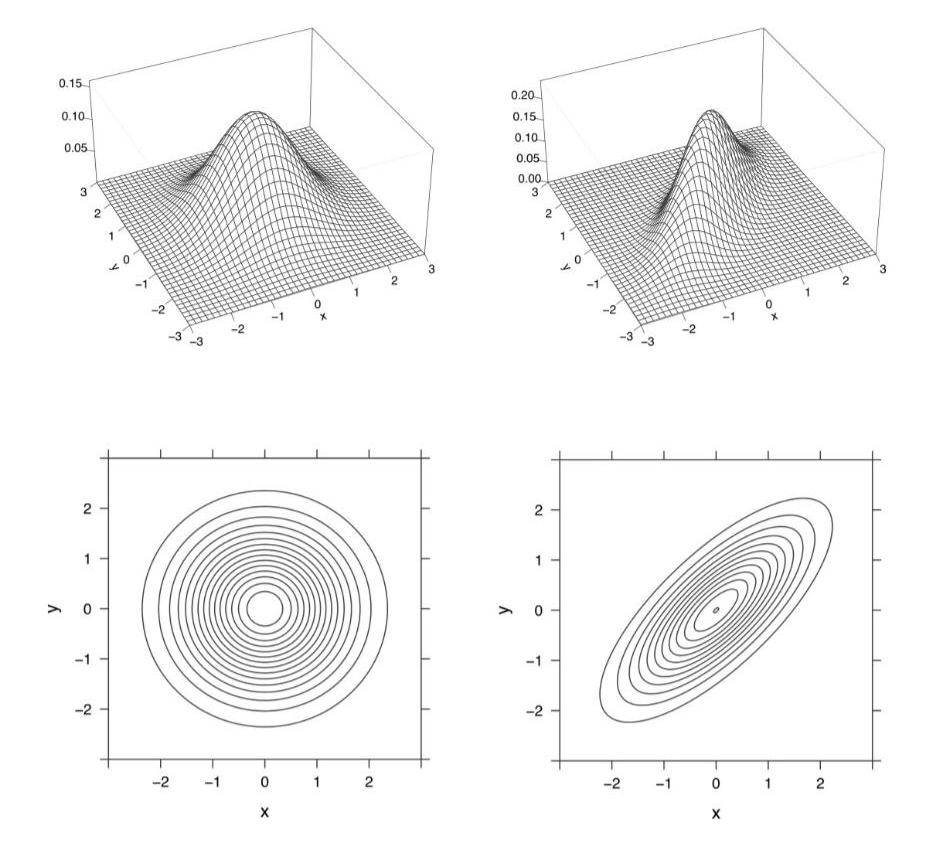
\includegraphics[width=1\linewidth]{images/bvn} \end{center}
\item
  The question is

  \begin{rmdbox}
  Are both of these considered {\hl{standard}} bivariate normals?

  \end{rmdbox}
\item
  From \href{https://en.wikipedia.org/wiki/Multivariate_normal_distribution\#Standard_normal_random_vector}{wikipedia}\footnote{Citing Lapidoth, Amos (2009). \emph{A Foundation in Digital Communication}. Cambridge University Press. ISBN 978-0-521-19395-5.}:

  \begin{quote}
  A real random vector ${\displaystyle \mathbf {X} =(X_{1},\ldots ,X_{k})^{\mathrm {T} }}$ is called a standard normal random vector if all of its components ${\displaystyle X_{k}}$ are independent and each is a zero-mean unit-variance normally distributed random variable, i.e.~if ${\displaystyle X_{k}\sim \ {\mathcal {N}}(0,1)}$ for all ${\displaystyle k}$.
  \end{quote}
\item
  For any RVs $X$ and $Y$, independence implies $\rho = 0$. So, according to this definition, the {\hl{standard bivariate normal}} has PDF

  \[
  f(x, y) = \frac{1}{2\pi} \cdot 
  \exp\left(
    -\frac{1}{2} \cdot (x^2 + y^2)
  \right)
  \]

  and {\hl{corresponds only to the graphs on the left}}.
\item
  In the general case, for $X \sim \mathcal N\left(\mu_X, \sigma^2_X\right)$, and $Y \sim \mathcal N\left(\mu_Y, \sigma^2_Y\right)$ and with $\rho \neq 0$, the PDF is

  \begin{multline}
  f(x,y) = \\ 
  {
    \frac {1}
    {
      2\pi \sigma _{X}\sigma _{Y}\tau
    }
  }\cdot \exp \left(
    -{
      \frac {1}{2\tau^2}
    }\left[
      \left(
        {\frac {x-\mu _{X}}{\sigma_{X}}}
      \right)^{2} -
      2\rho \left(
        {\frac {x-\mu _{X}}{\sigma_{X}}}
      \right)
      \left(
        {\frac {y-\mu _{Y}}{\sigma_{Y}}}
      \right) +
      \left(
        {\frac {y-\mu _{Y}}{\sigma_{Y}}}
      \right)^{2}
    \right]
  \right)
  \end{multline}

  with $\tau = \sqrt{1 - \rho^2}$ as before.
\item
  The PDF of the conditional distribution of $X$ given $Y = y$ is

  \[
  f_{X \mid Y} (x, y) = 
  \frac{f(x, y)}{f_Y(y)}
  \]

  where $f_Y$ is the marginal PDF

  \[
  \begin{aligned}
  f_Y(y) &= \int_{-\infty}^\infty f(x, y)\, dx \\
  &= \frac{1}{\sigma_Y \sqrt{2\pi}} 
     \cdot 
     \exp\left( -(y - \mu_Y)^2 / 2 \sigma_Y^2 \right)
  \end{aligned}
  \]

  yielding

  \[
  \begin{aligned}
  f_{X \mid Y} (x, y) 
  &= \frac{f(x, y)}{f_Y(y)} \\
  &= \frac{
    {
      \frac {1}
      {
        2\pi \sigma _{X}\sigma _{Y}\tau
      }
    }\cdot \exp \left(
      -{
        \frac {1}{2\tau^2}
      }\left[
        \left(
          {\frac {x-\mu _{X}}{\sigma_{X}}}
        \right)^{2} -
        2\rho \left(
          {\frac {x-\mu _{X}}{\sigma_{X}}}
        \right)
        \left(
          {\frac {y-\mu _{Y}}{\sigma_{Y}}}
        \right) +
        \left(
          {\frac {y-\mu _{Y}}{\sigma_{Y}}}
        \right)^{2}
      \right]
    \right)
  }{
    \frac{1}{\sigma_Y \sqrt{2\pi}} 
       \cdot 
       \exp\left( -(y - \mu_Y)^2 / 2 \sigma_Y^2 \right)
    } 
  \\
  \end{aligned}
  \]
\end{itemize}

\hypertarget{references}{%
\chapter*{References}\label{references}}
\addcontentsline{toc}{chapter}{References}

\hypertarget{refs}{}
\begin{CSLReferences}{1}{0}
\leavevmode\vadjust pre{\hypertarget{ref-JosephK.Blitzstein989}{}}%
Blitzstein, Joseph K., and Jessica Hwang. 2019. \emph{Introduction to Probability, Second Edition}. CRC Press.

\leavevmode\vadjust pre{\hypertarget{ref-RobertP.Dobrow1345}{}}%
Dobrow, Robert P. 2016. \emph{Introduction to Stochastic Processes with {R}}. John Wiley \& Sons.

\end{CSLReferences}

\end{document}
